% -*- TeX-master: "../all_the_notes.tex" -*-
\newpage
\section{Dipole          operator          for          coupling          \cite{Astafiev2010}
  \cite{abdumalikov2010} \label{sec:dipole_coupling}}

\begin{framed}\noindent
  \textbf{Premise}

  We examine driving close to \iket{i}\ilra\iket{j}.
\end{framed}

\begin{minipage}[l]{0.5\linewidth}%
  %% Capacitive
  \begin{framed}\noindent
    \begin{equation}\label{eq:couple1}
      \begin{aligned}
        \hbar\Omega_{ij}\grey{\cos(\omega_{ij}t)} = \blue{\vartheta_{ij}}\iabs{V_\text{mw}}\grey{\cos(\omega_{ij}t)} & \\
        \blue{\vartheta_{ij} = C_\text{q-mw}V_\text{qubit}\zeta_{ij}} &
      \end{aligned}
    \end{equation}

    \begin{itemize}
    \item $ \iabs{V_\text{mw}} $:\hfill voltage amplitude in the transmission line;
    \item $ C_{q-mw} $:\hfill mutual capacitance between the line and qubit;
    \item $ V_\text{qubit} $:\hfill persitent voltage on the qubit;
    \item $ \zeta = \begin{pmatrix}
        \bra{0}\hat{A}\ket{0} & \bra{0}\hat{A}\ket{1} & \cdots\\
        \bra{1}\hat{A}\ket{0} & \bra{1}\hat{A}\ket{1} & \cdots\\
        \vdots & \vdots & \ddots
      \end{pmatrix} $:\hfill normalised (to unity) matrix elements.
    \end{itemize}%
  \end{framed}%
\end{minipage}%
\begin{minipage}[r]{0.5\textwidth}
  %% Inductive
  \begin{framed}\noindent

    \begin{equation}\label{eq:couple7}
      \begin{aligned}
        \hbar\Omega_{ij}\grey{\cos(\omega_{ij} t)} = \red{\vartheta_{ij}}\iabs{I_{mw}}\grey{\cos(\omega_{ij} t)}&  \\
        \red{\vartheta_{ij} = MI_p\zeta_{ij}} &
      \end{aligned}
    \end{equation}

    \begin{itemize}
    \item $ \iabs{I_{mw}} $:\hfill current amplitude in the transmission line;
    \item M:\hfill mutual inductance between the line and qubit;
    \item $ I_p $:\hfill persitent current in the loop;
    \item $ \zeta = \begin{pmatrix}
        \bra{0}\hat{A}\ket{0} & \bra{0}\hat{A}\ket{1} & \cdots\\
        \bra{1}\hat{A}\ket{0} & \bra{1}\hat{A}\ket{1} & \cdots\\
        \vdots & \vdots & \ddots
      \end{pmatrix} $:\hfill normalised (to unity) matrix elements.
    \end{itemize}

  \end{framed}
\end{minipage}
\begin{figure}[h]
  \centering 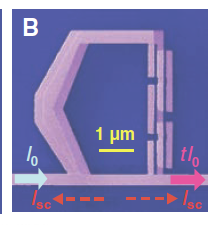
\includegraphics[height=4cm]{oleg_mutual}
\end{figure}

\noindent

\newpage

\begin{minipage}{0.5\linewidth}%
  %% Capacitive
  \begin{enumerate}%
  \item Writing out the charging energy in the  qubit, due to the qubits, $ Q_\text{qubit} $,
    and induced capacitively charges:

    \begin{equation}\label{eq:couple2} {\scriptsize
      \begin{aligned}
        E_C & = \frac{Q_\text{total}^2}{2C_\text{total}}\\
        & = \frac{1}{2C_\text{total}}\bigg[Q_\text{qubit} + {C_\text{q-r}V_{mw}}\bigg]^2\\
        & = {\frac{1}{2C_\text{total}}\bigg[Q_\text{qubit}^2 + \red{2Q_\text{qubit}C_\text{q-mw}V_\text{mw}} + C_\text{q-mw}^2V_\text{mw}^2\bigg]}\\
      \end{aligned}}
  \end{equation}
  \noindent Only the red terms are of interest for interaction, since they link the qubit and
  microwave systems.\red{Therefore only the red one is carried on}.

\item \begin{equation}\label{eq:couple3}
    \begin{aligned}
      E_c & = \frac{Q_\text{qubit}}{C_\text{total}}C_\text{q-mw}V_\text{mw}\\
      & = V_\text{qubit}C_\text{q-mw}V_\text{mw},
    \end{aligned}
  \end{equation}
  \noindent   where  we   have  the   residual  voltage   from  the   charge  on   the  qubit
  $ V_\text{qubit} $.

\item Now  let us take the  quantum mechanical operators  and evaluate with the  qubit states
  (which \textbf{do not} act on the microwave line operator $ \hat{V}_{mw} $):
  \begin{equation}\label{eq:couple4}
    \begin{aligned}
      \mathcal{H}_{int} & = \hat{V}_\text{qubit}\hat{C}_\text{q-r}\hat{V}_{mw} \\
      & = \sum_{i,j}\iketbra{i}{j}\blue{\bra{i}\hat{C}_{qr}\hat{V}_{\text{qubit}}\ket{j}} \hat{V}_{mw}\\
      & = \sum_{i,j}\iketbra{i}{j}\blue{\vartheta_{ij}} \hat{V}_{mw}\\
    \end{aligned}
  \end{equation}
\end{enumerate}
\end{minipage}%
\begin{minipage}{0.5\linewidth}%
  %% Inductive
  \begin{enumerate}%
  \item Writing out the  flux energy in the qubit, due to the  qubits, $ \Phi_\text{qubit} $,
    and induced, $ M_I $ magnetic fluxes:

    \begin{equation}\label{eq:couple8}{\scriptsize
      \begin{aligned}
        E_\Phi &= \frac{\Phi_\text{total}^2}{2L}\\
        & = \frac{1}{2L_{\text{total}}}\bigg[\Phi_\text{qubit} + MI_{mw}\bigg]^2\\
        &        =       \frac{1}{2L_\text{total}}\bigg[\Phi_\text{qubit}^2        +
        \red{2\Phi_\text{qubit}MI_{mw}} + M^2I_{mw}^2\bigg]
      \end{aligned}}
  \end{equation}
  \noindent Only the red terms are of interest for interaction, since they link the qubit and
  microwave systems.\red{Therefore only the red one is left}.

\item \begin{equation}\label{eq:couple9}
    \begin{aligned}
      E_\Phi &= \frac{\Phi_\text{qubit}}{L_\text{total}}MI_{mw}\\
      & = I_pMI_{mw}
    \end{aligned}
  \end{equation}

  \noindent where we added the persistent current in the loop $ I_p $.

\item Now  let us  take the  quantum mechanical  operators and  evaluare the  matrix elements
  \cite{Astafiev2010}:
  \begin{equation}\label{eqn:dipole_1}
    \begin{aligned}
      \mathcal{H}_{int} & = \hat{I}_{mw}\hat{M}\hat{I}_p\\
      & = \sum_{i,j}\iketbra{i}{j}\red{\bra{i}\hat{M}\hat{I}_p\ket{j}} \hat{I}_{mw}\\
      & = \sum_{i,j}\iketbra{i}{j}\red{\vartheta_{ij}} \hat{I}_{mw}\\
    \end{aligned}
  \end{equation}

\item \begin{equation}\label{eq:couple10} \red{\vartheta_{ij} = MI_p\zeta_{ij}}.
  \end{equation}

  \noindent  \red{Effectively  the  atom  transitions  from 1  persistent  current  state  to
    another.}

  Adding a  matrix element  factor, so  that only a  change of  state (\iket{0}\ilra\iket{1})
  generates a change

    \begin{equation}\label{eq:couple13}
      \iabs{MI_p}\zeta_{ij}.
    \end{equation}

  \end{enumerate}
\end{minipage}

\newpage

\begin{framed}
  \noindent Dispelling common myths: so what is the difference between

  \begin{equation}
    \label{eq:myth1}
    \delta A = \ibra{e}\hat{A}\iket{e} - \ibra{g}\hat{A}\iket{g} \qquad \text{and} \qquad \ibra{e}\hat{A}\iket{g}
  \end{equation}

  \noindent Well, it comes down to what elements you need from the interaction matrix:

  \begin{center}
    \includegraphics[height=4cm]{matrix_coupling}

    {\small These cross terms can be used in perturbation theory\label{fig:matrix_coupling}}
  \end{center}

\end{framed}
\begin{enumerate}

\item  $ \mathbf{\hat{V}_\text{qubit}}  $ is  the  qubit voltage  operator, which  next to  a
  transition reads

  \begin{equation}\label{eq:couple5}
    \hat{V}_\text{qubit} = \frac{2e}{C_\text{total}}\sigma_x.
  \end{equation}

\item $ \mathbf{\hat{V}_\text{mw}} $ is the microwave field operator
  \begin{equation}\label{eq:couple6}
    {\hat{V}_\text{mw} = \iabs{V_{\text{mw}}}\cos(\omega t)\bigg(a^\dagger +a\bigg)}
  \end{equation}
\item Fully we have

  \begin{equation}
    \begin{aligned}
      H_{int}&=2e\frac{\hat{C}_\text{q-mw}}{C_\text{total}}\iabs{V_{\text{mw}}}\cos(\omega t)\sigma_x\\
      &= \hbar\Omega\cos(\omega t)\sigma_x.
    \end{aligned}
  \end{equation}
\end{enumerate}

\begin{framed}\noindent
  \begin{equation}
    \mathcal{H}_{\text{int}}=g_0\big(\sigma^++\sigma^-\big)\big(a+a^\dagger\big),          \qquad
    g_0=V_{q0}C_{qr}V_{r0},
  \end{equation}
\end{framed}

\begin{enumerate}


\item  Now,  to express  the  value  $  \hat{I}_{mw}  = \iabs{I_{mw}}\cos(\omega_dt)$  as  an
  operator, we follow these reasons:
  \begin{itemize}
  \item The current which supplied the energy couples the
  \end{itemize}
  \noindent to get
  \begin{equation}\label{eq:couple15}
    \hat{I}_{mw} = \iabs{I_{mw}}\cos(\omega_{ij}t)\bigg(a + a\idagger\bigg).
  \end{equation}
\end{enumerate}

\begin{framed}\noindent
  So alltogether, the operator on the qubit system is
  \begin{equation}\label{eq:couple16}
    \begin{aligned}
      \mathcal{H}_{int} & = \sum_{i,j}{\bigg[\iabs{I_{mw}}\vartheta_{ij}\cos(\omega_{ij}t)\bigg]}\iketbra{i}{j}\\
      & = \sum_{i,j} \hbar\Omega_{ij} \cos(\omega_{ij}t) \iketbra{i}{j}\qquad \red{\hbar\Omega_{ij} = \iabs{I_{mw}}MI_p\zeta_{ij}}\\
    \end{aligned}
  \end{equation}

\end{framed}



\subsection{Summary \cite{Astafiev2010}}
\begin{framed}\noindent
  \noindent When a qubit system emits, the  strength of emission depends on the dipole moment
  of the system, as we saw in Chapter~\ref{sec:dipole_coupling}:
  \begin{equation}\label{eq:couple17}
    \vartheta_{ij} = \left[\begin{aligned}
        & \blue{C_{q-mw}V_\text{qubit}\zeta_{ij}} \qquad&& \text{\blue{capacitive coupling causes induced charge}}\\
        & \red{MI_p\zeta_{ij}} \qquad&& \text{\red{inductive coupling causes induced flux}}
      \end{aligned}\right.
  \end{equation}
\end{framed}

\noindent adding some  time dependence of $  \omega $, \textbf{since the system  will repospond at
  the rate of out driving}, and expanding out the matrix elements for a two level system

\begin{equation}\label{eq:couple18}
  \zeta = \begin{pmatrix}
    \bra{0}\hat{A}\ket{0} & \bra{0}\hat{A}\ket{1} \\
    \bra{1}\hat{A}\ket{0} & \bra{1}\hat{A}\ket{1} \\
  \end{pmatrix} \ira \begin{pmatrix} 0 & \red{\isigmaminus}\\\isigmaplus&0
  \end{pmatrix}
\end{equation}

\noindent we can concentrate on the \red{relaxation} matrix element to get

\begin{equation}\label{dipole_2level}
  \vartheta_{ij}(t) = MI_p\isigmaminus e^{-i\omega t}
\end{equation}

\newpage
